The standard Beta-wavelet bank built on the unsigned Laplacian $\bm{L}$ captures the anomaly signal by detecting the right-shift of the spectral energy \citep{BWGNN}.
However, every observed edge is treated as homophilous and therefore smooths the signal propagation.
In the neighborhoods of anomaly nodes, the heterophily property of the edges adds more information to the filter and can be exploited to detect the abnormal signal.
%Consequently, this setting allows heterophilous connections to leak abnormal signal into normal neighborhoods.
Built upon this motivation, our proposed ESO-GAD introduces the local semantics of the edges into the Beta-wavelet filter by using a signed spectral operator (Fig.~\ref{fig:framework}).
In the edge-calibrated phase, we form an edge descriptor from the features of the two endpoints and train a lightweight classifier.
The resulting classifier predicts the heterophily probability of an edge $(u,v)$, which is the probability that $u$ and $v$ carry different labels.
In the learning phase, the predicted probabilities are then mapped to soft edge signs, which turn the input graph into a weighted signed graph and induce a signed normalized Laplacian $\bm{L}_{\eta}$.
To control the effect of the edge estimator's bias, a learnable calibration strength $\eta$ is introduced to $\bm{L}_{\eta}$ .
We then construct a localized Beta-wavelet filter bank on $\bm{L}_{\eta}$, whose band-pass channels now separate the low- and high-frequency components of the signed spectrum. 
The channel responses are then aggregated through a learnable simplex gate and used to learn the target labels.
\begin{figure*}[ht]
\centerline{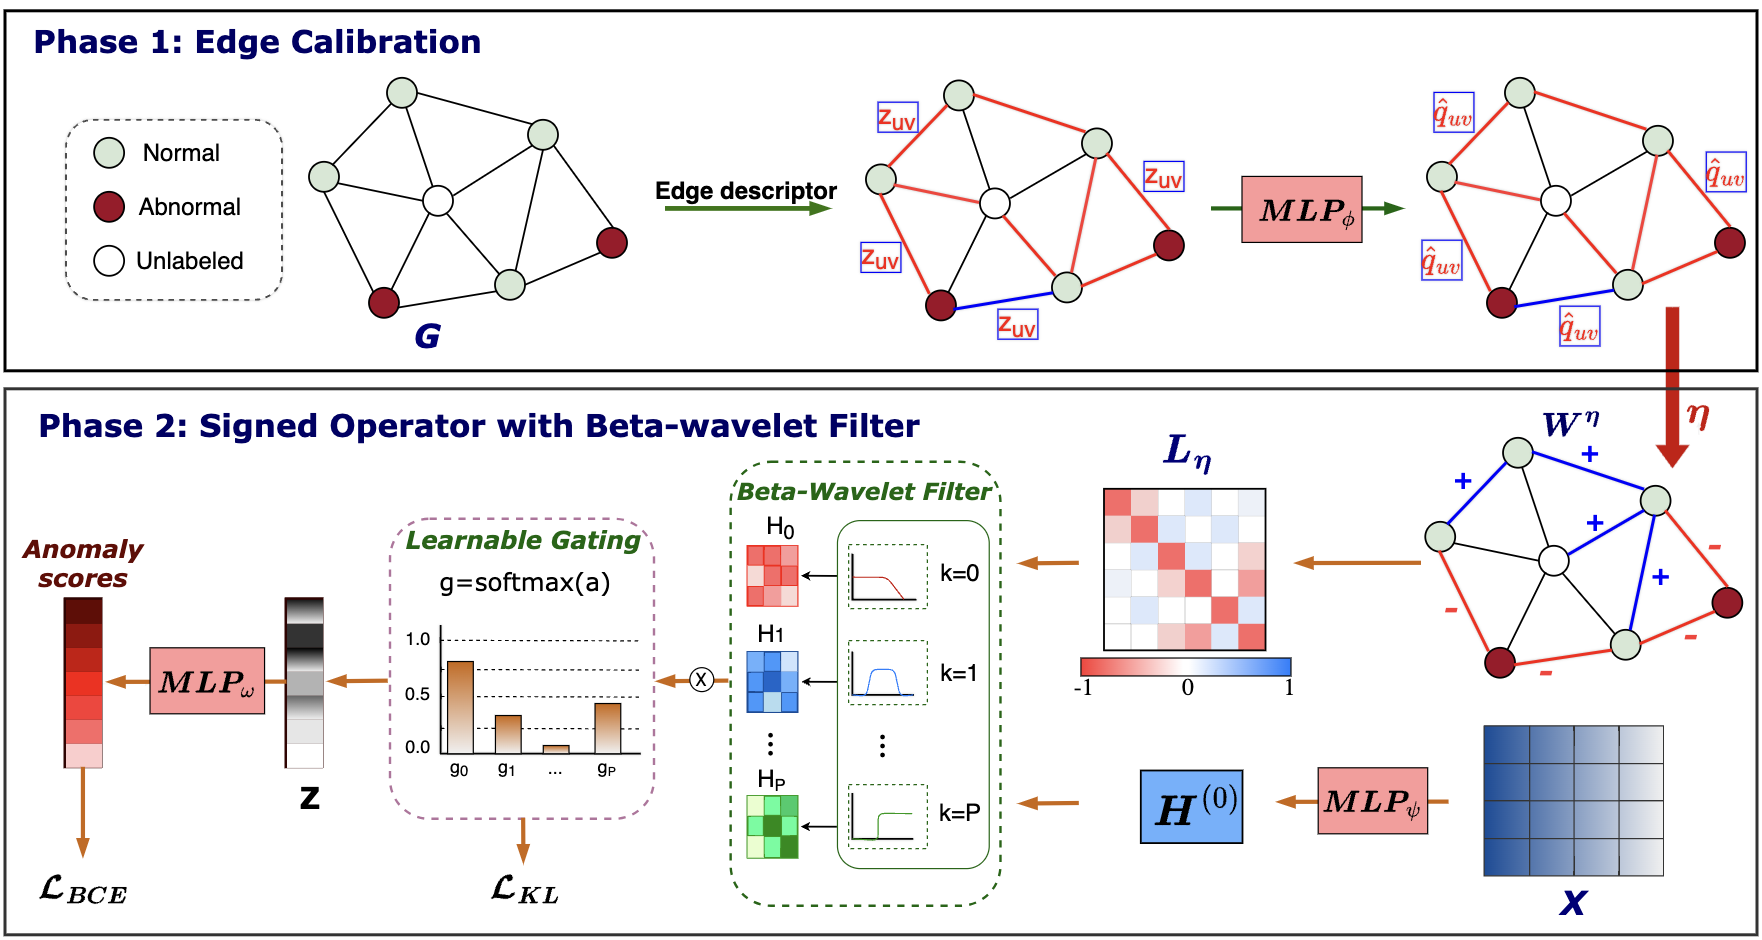
\includegraphics[width=0.9\linewidth]{images/pipeline3.png}}
\caption{Overview of our proposed ESO-GAD with two main phases. The edge calibration phase trains an estimator parameterized by $\phi$ with K-fold cross-fitting to predict the heterophily score $\hat{q}_{uv}$. The second phase constructs a signed spectral operator on the calibrated signed weights and learns to predict the anomaly nodes, with a KL-regularized aggregator.} 
\label{fig:framework}
% \vspace{-10pt}
\end{figure*}